\documentclass[a4paper, 12pt]{article}
\usepackage{geometry}
\usepackage[russian]{babel}
\usepackage[T2A]{fontenc}
\usepackage{chngcntr}
\usepackage{graphicx}
\usepackage{verbatim}

\begin{document}


\begin{titlepage}

\begin{center}
{\textsc{\textbf{Правительство Российской Федерации}}}\\
\vspace{0.5cm}
\hrule
\vspace{0.5cm}
{\textsc{Федеральное государственное автономное образовательное учреждение\\высшего образования <<Национальный исследовательский университет\\<<Высшая школа экономики>>}}\\
\vspace{1cm}
Кафедра <<Компьютерная безопасность>>
\end{center}

\vspace{\fill}

\begin{center}
{\Large{\textbf{ОТЧЕТ \\ К ЛАБОРАТОРНОЙ РАБОТЕ №2}}} \\
\vspace{1em}
{\textbf{по дисциплине}} \\
\vspace{1em}
{\large{\textbf{<<Языки программирования>>}}}
\end{center}

\vspace{\fill}


\begin{flushright}
  \begin{minipage}[center]{15cm}

    \begin{minipage}[left]{5cm}
      {Работу выполнил\\студент группы СКБ-222}
    \end{minipage}
    \begin{minipage}[center]{5cm}
      \vspace{1.25cm}
      \hrulefill\\[-1cm]
      \begin{center}{подпись, дата}\end{center}
    \end{minipage}
    \begin{minipage}[right]{4cm}
      \vspace{0.4cm}
      \begin{flushright}{А.С. Куркотов}\end{flushright}
    \end{minipage}
    \\
    \\
    \\
    \begin{minipage}[left]{5cm}
      {Работу проверил}
    \end{minipage}
    \begin{minipage}[center]{5cm}
      \vspace{1.25cm}
      \hrulefill\\[-1cm]
      \begin{center}{подпись, дата}\end{center}
    \end{minipage}
    \begin{minipage}[right]{4cm}
      \begin{flushright}{С.А. Булгаков}\end{flushright}
    \end{minipage}
  \end{minipage}
\end{flushright}

\vspace{\fill}

\begin{center}
Москва~2022
\end{center}
\end{titlepage}
\setcounter{page}{2}
\setcounter{secnumdepth}{5}
\setcounter{tocdepth}{5}

\tableofcontents
\cleardoublepage

\setcounter{section}{1}
\counterwithout{subsection}{section}
\graphicspath{ {./images/} }

\cleardoublepage
\section*{Постановка задачи}\addcontentsline{toc}{section}{Постановка задачи}
Необходимо было разработать программу выполняющую интерактивное взаимодействие 
с пользовотелем: запрос данных и проверку корректности ввода.

Программа должна была состоять из основной функции и одной или более вспомогательных.

Также было нужно разработать вспомогательную функцию, позволяющую вводить элементы 
целочисленного массива, выводящую приглашение пользователю к вводу элемента под указанным
номером, с предусмотрением некорректного ввода пользователя и повторным приглашением
к вводу в таком случае. Функция ничего не должна возвращать. Функция должна принимать на вход
массив для заполнения и количество элементов в нём

Поскольку остальной функционал программы был оставлен на усмотрение исполнителя, 
я выбрал программу, проверяющую, являются ли целыми числами некоторое вводимое
пользователем число значений.
\cleardoublepage



\section*{Основная часть}\addcontentsline{toc}{section}{Основная часть}

\subsection{Описание вспомогательной стркутуры}
Для безопасной обработки ошибок без завершения программы была создана вспомогательная
стркутура \textit{intResult}, содержащая значение \textit{val}, хранящее "полезное" значение
и контрольные значение ошибки с её текстом

\subsection{Описание вспомогательных функций}
\subsubsection{Очистка буфера ввода}
Вызывается после обнаружения некорректного ввода пользователя
и считывает данные из буфера ввода, пока не дойдет до переноса строки. Функция
ничего не принимает и не возвращает.


\subsubsection{Инициализация структуры}
Вызывается при создании вспомогательной структуры. Задаёт все поля нулевыми
значениями. Ничего не принимает и не возвращает.


\subsubsection{Создание ошибки ''Введено не натуральное число''}
Вызывается, если пользователь ввёл значение, не являющееся натуральным числом.
Функция принимает указатель на вспомогательную структуру, задаёт значение \textit{error}
единицей и заполняет текст ошибки, ничего не возвращая.


\subsubsection{Создание ошибки ''Отсутствует ввод''}
Вызывается, если пользователь не ввёл значение. Функция принимает указатель 
на вспомогательную структуру, задаёт значение \textit{error}
единицей и заполняет текст ошибки, ничего не возвращая.


\subsubsection{Считывание целочисленного ввода}
Вызывается при вводе пользователем целого числа. Проверяет, что значение корректно, в
противном функции вызывает функцию 2.3 или 2.4. Функция ничего не принимает, и, вне зависимости от
наличия ошибки, возвращает вспомогательную структуру с результатом ввода.


\subsubsection{Вывод меню и валидация ввода}
Вызывается после выбора пользователем размера массива. Выводит приглашение к вводу
числа с соответствующим номером, считывает ввод при помощи функции 2.5, в случае наличия
ошибки повторяет приглашение ко вводу и выводит информацию об ошибке. Функция принимает
массив вводимых значений и его размер, и ничего не возвращает.


\subsection{Описание основной функции}
Основная функция считывает количество чисел, которые пользователь хочет ввести и
создаёт массив соответствующего размера, после чего вызывает функцию 2.6. После
окончания работы программы освобождает память, занятую массивом.



\subsection{Проверка результатов тестирования}


\subsubsection{Проверка базового функционала}


\paragraph{Проверка запроса размера массива}\mbox{}\\
При запуске программы должно выводиться приглашение пользователю ввести размер
массива, который он желает заполнить.\\
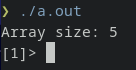
\includegraphics{arr_size_print.png}


\paragraph{Считывание и валидация чисел}\mbox{}\\
После ввода размера, пользователь должен ввести n чисел,
где n - размер массива. Каждый раз он должен видеть номер
вводимого числа.\\
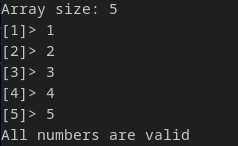
\includegraphics{input_accrept.png}


\subsubsection{Проверка обработки ошибок}
\paragraph{Отсутствует значение размера}\mbox{}\\
Если пользователь не предоставит значение размера,
программа попросит его ввести какое-либо значение для проверки.\\
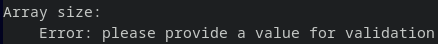
\includegraphics{no_input_size.png}


\paragraph{Значение размера нулевое}\mbox{}\\
Если пользователь введёт значение размера, равное 0,
программа попросит его ввести другое значение.\\
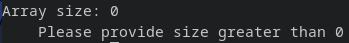
\includegraphics{zero_size.png}


\paragraph{Не натуральное значение размера}\mbox{}\\
Если пользователь введёт значение размера, не являющееся натуральным числом,
программа попросит его ввести натуральное значение.\\
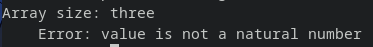
\includegraphics{non_natural_size.png}


\paragraph{Отсутствует число для валидации}\mbox{}\\
Если пользователь не введёт значение для проверки,
программа попросит его повторно ввести это значение.\\
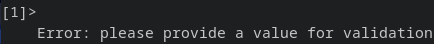
\includegraphics{no_input_validate.png}


\paragraph{Не натуральное число для валидации}\mbox{}\\
Если пользователь введёт не натуральное значение,
программа попросит его повторно ввести это значение.\\
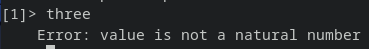
\includegraphics{non_natural_input_validate.png}


\cleardoublepage

\section*{Приложение A}\addcontentsline{toc}{section}{Приложение А}
\renewcommand\thesection{\Alph{section}}
\renewcommand\thesubsection{\thesection.\arabic{subsection}}
\setcounter{subsection}{0}

\subsection{Блок-схема \textit{clearStdin}}
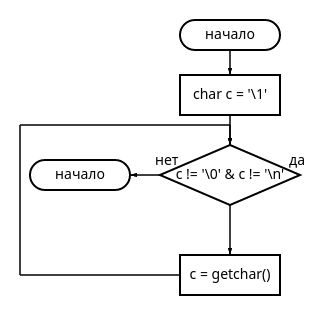
\includegraphics[width=\columnwidth]{clearStdin.png}

\subsection{Блок-схема \textit{initRes}}
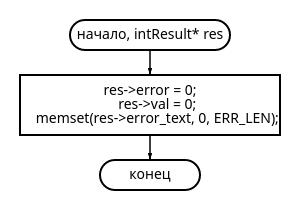
\includegraphics[width=\columnwidth]{initRes.png}

\subsection{Блок-схема \textit{nonNaturalRes}}
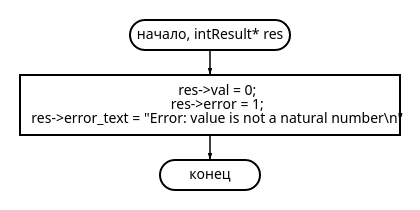
\includegraphics[width=\columnwidth]{nonNaturalRes.png}

\subsection{Блок-схема \textit{noInputRes}}
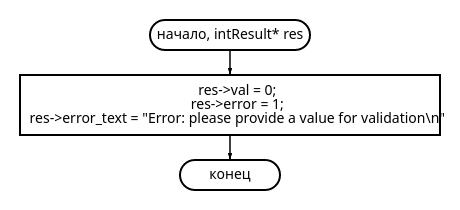
\includegraphics[width=\columnwidth]{noInputRes.png}

\subsection{Блок-схема \textit{getInt}}
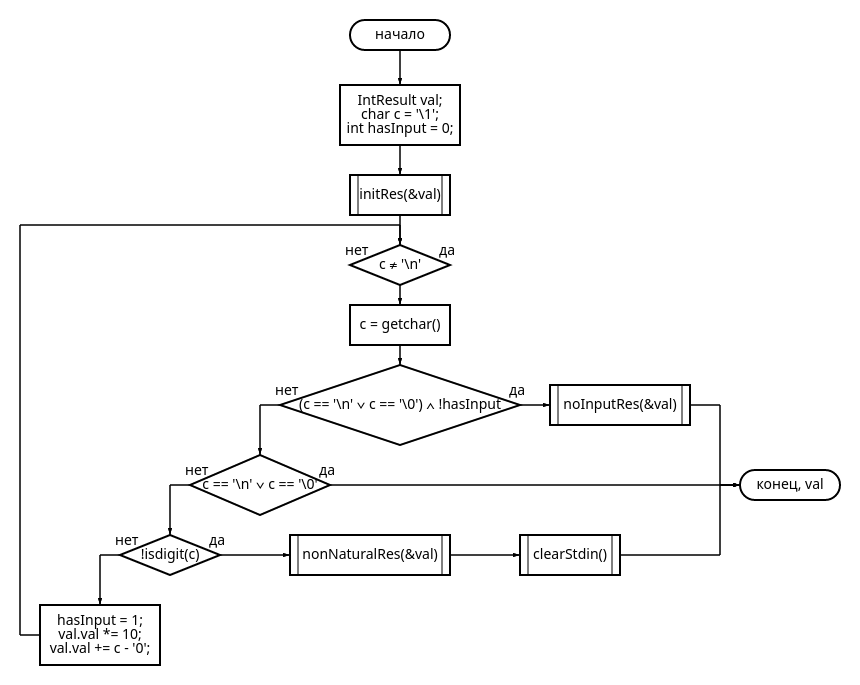
\includegraphics[width=\columnwidth]{getInt.png}

\subsection{Блок-схема \textit{validate}}
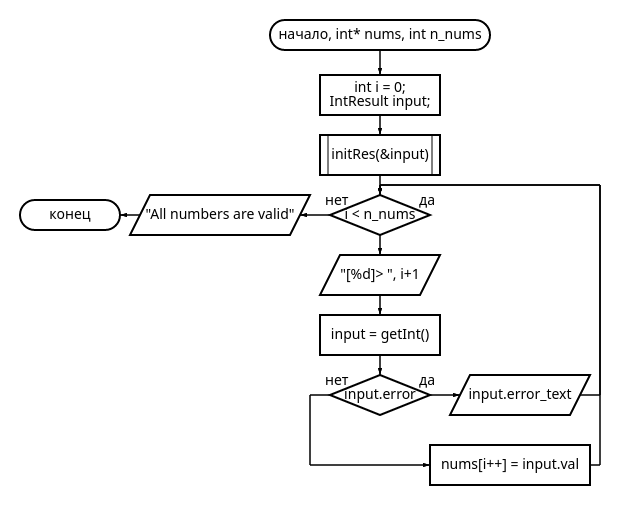
\includegraphics[width=\columnwidth]{validate.png}

\subsection{Блок-схема \textit{main}}
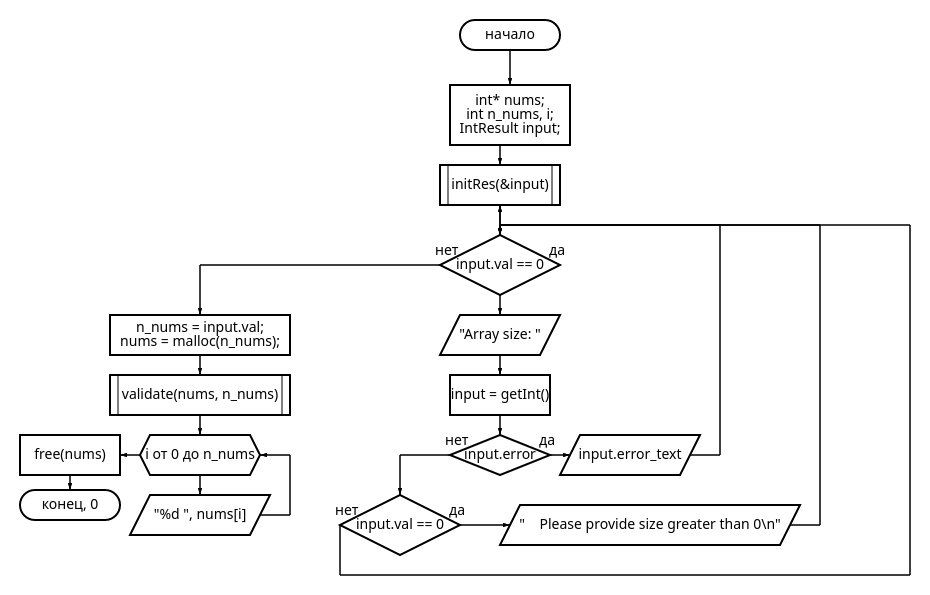
\includegraphics[width=\columnwidth]{main.png}


\cleardoublepage


\section*{Приложение B}\addcontentsline{toc}{section}{Приложение B}
\subsection{Код программы}

\fontsize{9}{9}\selectfont
\begin{verbatim}
#include <stdio.h>
#include <stdlib.h>
#include <string.h>
#include <ctype.h>

#define ERR_LEN 100

typedef struct {
    int val;
    int error;
    char error_text[ERR_LEN];
} IntResult;

void clearStdin() {
    char c = '\1';
    while (c != '\0' && c != '\n') c = getchar();
}

void initRes(IntResult* res) {
    res->error = 0;
    res->val = 0;
    memset(res->error_text, 0, ERR_LEN);
}

void nonNaturalRes(IntResult* res) {
    res->val = 0;
    res->error = 1;
    strcpy(res->error_text, "    Error: value is not a natural number\n");
}

void noInputRes(IntResult* res) {
    res->val = 0;
    res->error = 1;
    strcpy(res->error_text, "    Error: please provide a value for validation\n");

}

IntResult getInt() {
    IntResult val;
    char c = '\1';
    int hasInput = 0;

    initRes(&val);
    
    while (c != '\n') {
        c = getchar();
        
        if ((c == '\n' || c == '\0') && !hasInput) {
            noInputRes(&val);
            break;
        }
        if (c == '\n' || c == '\0') break;
        if (!isdigit(c)) {
            nonNaturalRes(&val);
            clearStdin();
            break;
        }

        hasInput = 1;
        val.val *= 10;
        val.val += c - '0';
    }

    return val;
}

void validate(int* nums, int n_nums) {
    int i = 0;
    IntResult input;
    initRes(&input);

    while (i < n_nums) {
        printf("[%d]> ", i+1);
        input = getInt();

        if (input.error){
            printf("%s", input.error_text);
            continue;
        }

        nums[i++] = input.val;
    }

    printf("All numbers are valid\n");
}

int main() {
    int* nums;
    int n_nums, i = 0;
    IntResult input;
    initRes(&input);

    while (input.val == 0) {
        printf("Array size: ");
        input = getInt();

        if (input.error) {
            printf("%s", input.error_text);
        } else if (input.val == 0) {
            printf("    Please provide size greater than 0\n");
        }
    }

    n_nums = input.val;
    nums = malloc(n_nums);

    validate(nums, n_nums);

    for (i = 0; i < n_nums; i++) {
        printf("%d ", nums[i]);
    }

    free(nums);
    return 0;
}
\end{verbatim}

\end{document}
